\subsection{GSTool}

Mit dem GSTOOL Programm vom BSI (Bundesamt für Sicherheit in der Informationstechnik) kann man entsprechende Sicherheitskonzepte
nach dem Verfahren des IT-Grundschutzes modellieren.
1994 wurde das IT-Grundschutzhandbuch veröffentlicht und nach 4 Jahren wurde das GSTOOL herausgegeben.
Die Verwendung von GSTOOL ist umsonst.

\subsubsection{Bewertung}

GUI des GSTOOLs ist übersichtlich und sehr nutzerfreundlich. Man kann sehr leicht die Komponenten finden und bedienen. Trotzdem gibt es keine Möglichkeit, die Netzpläne und Prozessflüsse darzustellen. Man kann auch nicht nur die doppelseitige Verlinkungen erstellen sondern auch die individuelle Beschreibungen. Was den Export von Berichten betrifft, besteht auch keine Möglichkeit.     

Wenn es um die Pflege und Weiterentwicklung geht, wird der Support nur bis Ende 2016 unterstützt. Deshalb steht in der Bewertung 0. 

Beim Support wurde nicht schnell auf die Emails geantwortet. Der Grund liegt vielleicht an der Weihnachtzeit.  



Die GSTOOL-Lizenzen sind frei für unmittelbare Bundes-, Landes- und Kommunalverwaltungen Deutschlands.
Einrichtungen der Forschung und Lehre bekommen einen Rabatt auf die unten genannten Preise.
Für alle anderen Besteller gilt folgende Preistabelle (Abbildung~\ref{fig:GSToolschema}).
Die gesamten Kosten, die die Tabelle darstellt, sind hoch im Vergleich mit anderen Lösungen. Daher gibt es 5 in der Tabelle, es stellt somit ebenfalls den Referenzwert dar.  


\begin{figure}[htbp]
	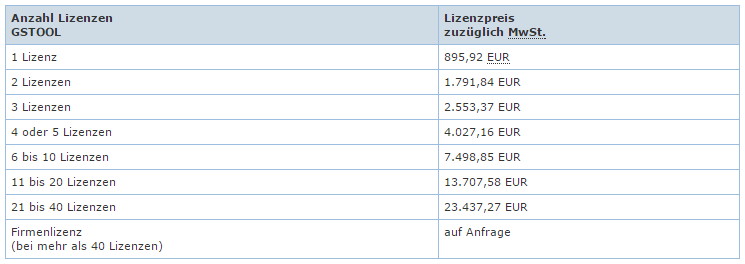
\includegraphics[scale=0.6]{images/gstoolpreis}
	\caption{Preise des GSTools}
	\label{fig:GSToolschema}
\end{figure}

Der Unterschied zwischen Hochschuleinsatz und Lehre ist nur $0.9\%$. Der Hochschuleinsatz hat $67.2\%$ und der Lehreinsatz $68.1\%$. Damit ist dieses Programm in fast gleichem Maß für beide Bereiche geeignet.

\subsubsection{Darstellung des Fallbeispiels}

Mithilfe des GSTOOls wurde das Beispiel der Hochschule modelliert. Das Beispiel ist in vollem Maß darstellbar, jedoch präsentiert das Programm den Baum nicht so ganz korrekt.  

\begin{figure}[htbp]
	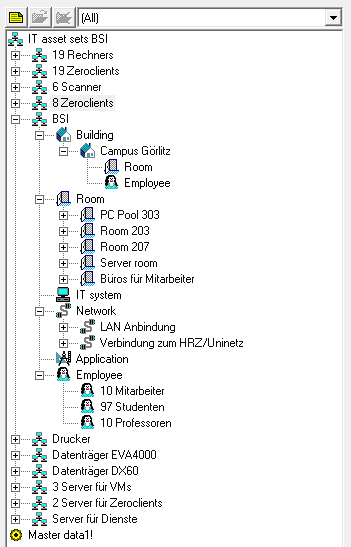
\includegraphics[scale=0.5]{images/gstooltree}
	\caption{Beispiel der Hochschule in GSTool}
	\label{fig:GSTooltree}
\end{figure}  


\begin{table}[h!bt]
%\centering
\begin{tabular}{|p{0.5\textwidth}|p{0.5\textwidth}|}
\hline 
Kriterium & Bewertung\\ 
\hline 
\textbf{GUI}& \\
\hline
Wizard & 7\\
\hline 
Infrastrukturdarstellung & 10 \\
\hline 
Netzpläne & 0 \\
\hline 
Prozessflüsse & 0 \\
\hline 
Schnelles Einpflegen von Änderungen & 10 \\
\hline
\textbf{Objektrelationen} & \\
\hline 
Doppelseitige Verlinkungen & 0 \\
\hline 
Vererbung & 10 \\
\hline 
Gruppierungen & 8 \\
\hline 
\textbf{Funktionalität} &\\
\hline 
Aktuelle BSI-Standards & 10 \\
\hline  
Erweiterbarkeit der Klassifizierungen & 10 \\
\hline 
Individuelle Beschreibungen & 0 \\
\hline 
Sicherheitsverstöße markieren & 10 \\
\hline
Bewertung des Sicherheitsstatus & 10 \\
\hline
Export von Berichten & 0 \\
\hline
BSI-Toolimport & 10 \\
\hline
Sicherheit des Tools an sich & 10 \\
\hline
Risikobewertung & 10 \\
\hline
\textbf{System}&  \\
\hline
Verteiltes Arbeiten & 10 \\
\hline
Rechtevergabe & 10 \\
\hline
Kosten & 5 \\
\hline
Support & 5 \\
\hline
Zertifizierung & 10 \\
\hline
Dokumentation & 7 \\
\hline
Marktpräsenz & 10 \\
\hline
Spezielle Zielgruppe & 8 \\
\hline
Pflege/Weiterentwicklung & 0 \\
\hline
\multicolumn{2}{c}{}\\
\hline
\textbf{Gesamt} & 190\\
\hline
Hochschuleinsatz & $67,2\%$\\
\hline
Lehre & $68,1\%$\\
\hline
\end{tabular} 
\caption{Bewertung: GSTool}
\label{tab:BewertungGSTool}
\end{table}